\section{Developing a GPU tridiagonal solver}

\begin{frame}
\frametitle{Requirements of tridiagonal solver}
\begin{columns}
\begin{column}{0.5\textwidth}
\begin{itemize}
\item For a 1-D grid, solution gives the derivative
    at all points simultaneously
\item For 2-D and 3-D grids,
    must solve many independent tridiagonal systems
\item Systems have the same tridiagonal coefficients,
    different right hand sides
\item Need a tridiagonal solver that solves
    a given system for several right hand sides
\item For 2-D problems $n \sim N_{rhs}$;
    for 3-D problems $n << N_{rhs}$
\end{itemize}
\end{column}
\begin{column}{0.5\textwidth}
    \hspace{1cm}
    \includegraphics[width=120px]{img/grid-lines.eps}
\end{column}
\end{columns}
\end{frame}

\begin{frame}
\frametitle{Thomas algorithm}
\begin{itemize}
\item Derived from Gaussian elimination
\item Requires $2n$ steps and $4n$ storage
\item The most efficient sequential algorithm
\item What about parallelization/GPUs?
    \begin{itemize}
        \item inherently sequential
        \item use multiple threads to solve
            individual tridiagonal systems
            (Sakharnykh et al.)
    \end{itemize}
\end{itemize}
\end{frame}

\begin{frame}
\frametitle{Issues in GPU implementation}
\begin{columns}
\begin{column}{0.5\textwidth}
\begin{itemize}
    \item Uncoalesced memory accesses
    \item Needs data rearrangement to coalesce accesses
    \item Does not expose enough parallelism
    \item $2n$ steps - can do better on GPU
    \item A case in which \emph{algorithm choice
        significantly impacts GPU performance}
\end{itemize}
\end{column}
\begin{column}{0.5\textwidth}
    \includegraphics[width=120px]{img/pThomas.eps}
\end{column}
\end{columns}
\end{frame}

\begin{frame}
\frametitle{Tridiagonal solvers for the GPU}
\begin{itemize}
\item Zhang et al. (2010) describe the implementation
    of three algorithms for tridiagonal systems on GPUs
    \begin{itemize}
        \item Cyclic reduction
        \item Parallel cyclic reduction
        \item Recursive doubling
    \end{itemize}
\item \textbf{Step efficient}: trade more work per step for \emph{fewer steps}
\item Exhibit \emph{fine-grained} parallelism - more suited to GPU
\item Subsequent efforts based on CR and PCR primarily
\end{itemize}
\end{frame}

\begin{frame}
\frametitle{Cyclic reduction}
\begin{columns}
\begin{column}{0.5\textwidth}
\begin{itemize}
\item Buzbee and Goleb (1970)
\item \textbf{Forward reduction} ($log_2(n)-1$ steps):
    \begin{itemize}
    \item Eliminate odd-indexed equations at each step
    \item Two-by-two system is left
    \end{itemize}
\item \textbf{Backward substitution} ($log_2(n)-1$ steps):
    \begin{itemize}
    \item Solve for odd-indexed equations using even-indexed values
    \end{itemize}
\item Best case ($n$ parallel threads): requires $2log_2(n)-1$ steps
\end{itemize}
\end{column}
\begin{column}{0.5\textwidth}
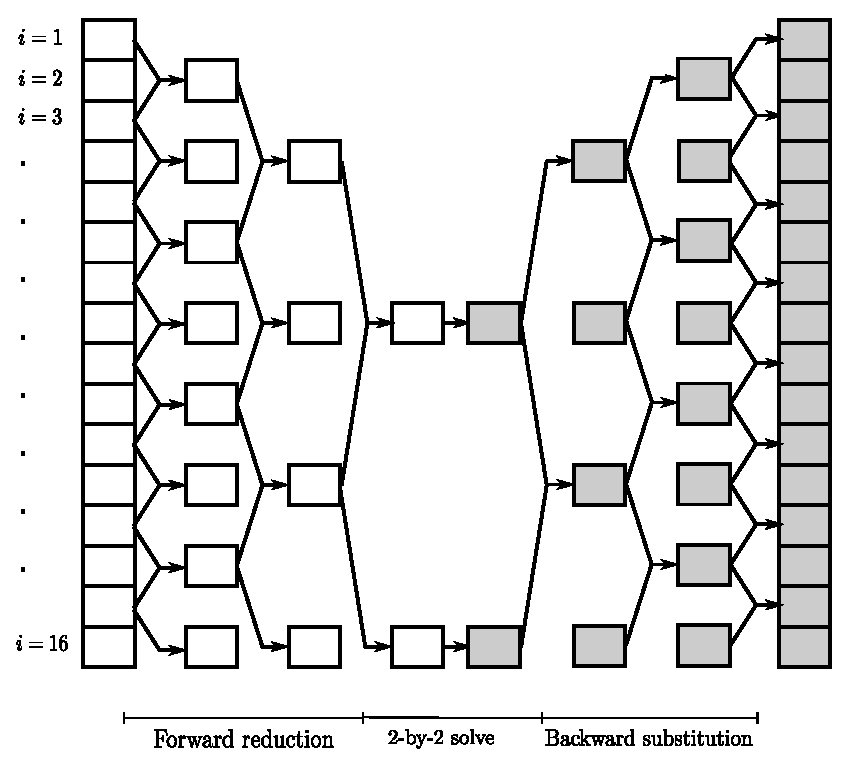
\includegraphics[width=150px]{img/cyclic-reduction.eps}
\end{column}
\end{columns}
\end{frame}

\begin{frame}
\frametitle{Cyclic reduction}
\begin{columns}
\begin{column}{0.5\textwidth}
\begin{itemize}
\item $17n$ operations,
    compared to $8n$ in Thomas algorithm
\item But exhibits more parallelism:
\begin{itemize}
    \item Individual systems can be solved independently
    \item Individual equations can be computed independently
\end{itemize}
\item Equations updated in place: $4n$ storage (same as Thomas algorithm)
\item Synchronization between threads required at each step
\end{itemize}
\end{column}
\begin{column}{0.5\textwidth}
\centering
Forward reduction

(diagonals $a$, $b$, $c$ and RHS $d$)
\scalebox{0.8}{
\vbox{
\begin{align*} 
    k_1 &= \frac{a_i}{b_{i-1}}, k_2 = \frac{c_i}{b_{i+1}} \\
    a^{\prime}_i &= -a_{i-1}k_1 \\
    b^{\prime}_i &= b_i - c_{i-1}k_1 - a_{i+1}k_2 \\
    c^{\prime}_i &= -c_{i+1}k_2 \\
    d^{\prime}_i &= d_i - d_{i-1}k_1  - d_{i+1}k_2 \\
\end{align*}}}

\centering
Backward substitution
\scalebox{0.8}{
\vbox{
\begin{align*}
x_i &= \frac{d^{\prime}_i - a^{\prime}_ix_{i-1} - \
    c^{\prime}_ix_{i+1}}{b^{\prime}_i}
\end{align*}}}
\end{column}
\end{columns}
\end{frame}

\begin{frame}
\frametitle{Issues in GPU implementation}
\footnotesize
\begin{columns}
\begin{column}{0.5\textwidth}
\begin{itemize}
    \item Strided memory access:
        stride increases by a factor of 2 at each step
        (decreases during backward substitution)
    \item \textbf{Solution}: use \emph{shared memory} (cache)
    \item Thread activity decreases during forward
        reduction and increases during backward substitution
    \item \textbf{Solution}: schedule threads for each step
        \begin{itemize}
            \footnotesize
            \item conflicts with shared memory usage
        \end{itemize}
    \item Shared memory \emph{bank conflicts}
        due to power-of-2 strides; reduced GPU occupancy
    \item We provide both implementations:
        global memory \emph{and} shared memory
\end{itemize}
\end{column}
\begin{column}{0.5\textwidth}
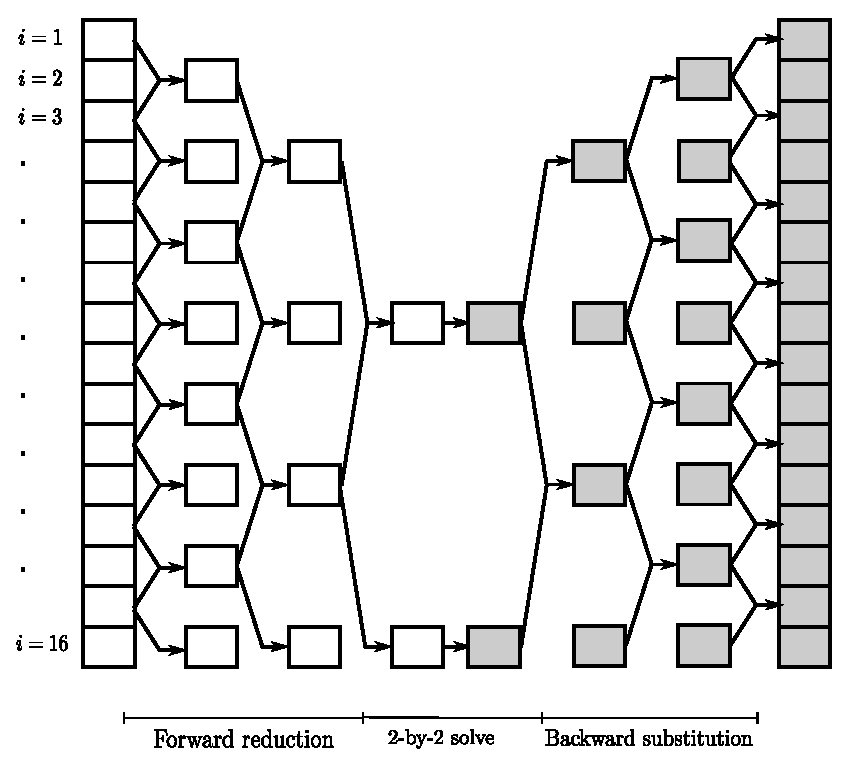
\includegraphics[width=150px]{img/cyclic-reduction.eps}
\end{column}
\end{columns}
\end{frame}

\begin{frame}
\frametitle{Efforts for improving performance}
\begin{itemize}
    \item Zhang et al.: hybrid CR+PCR solver
    \item G{\"o}ddeke et al.: separate even and odd indexed
        coefficients
    \item Davidson et al.: register packing
    \item Esfahanian et al.: global memory with data rearrangement
\end{itemize}
\end{frame}

\begin{frame}
\frametitle{A novel approach}
\begin{columns}
\begin{column}{0.5\textwidth}
\begin{itemize}
\item Solving system with same matrix and different RHS
\item Computing $a^\prime$, $b^\prime$ and $c^\prime$
    for each system and at every time step - \textbf{redundant}
\item Storing coefficients (similar to LU) - \textbf{expensive}
\item Approach: exploit the simple matrix structure
\end{itemize}
\end{column}
\begin{column}{0.5\textwidth}
\centering
Forward reduction
\scalebox{0.8}{
\vbox{
\begin{align*} 
    k_1 &= \frac{a_i}{b_{i-1}}, k_2 = \frac{c_i}{b_{i+1}} \\
    a^{\prime}_i &= -a_{i-1}k_1 \\
    b^{\prime}_i &= b_i - c_{i-1}k_1 - a_{i+1}k_2 \\
    c^{\prime}_i &= -c_{i+1}k_2 \\
    d^{\prime}_i &= d_i - d_{i-1}k_1  - d_{i+1}k_2 \\
\end{align*}}}
\end{column}
\end{columns}
\end{frame}

\begin{frame}
\frametitle{A novel approach}
\begin{columns}
\begin{column}{0.5\textwidth}
\begin{itemize}
\item Diagonals are nearly constant (\emph{near-Toeplitz tridiagonal})
\item Symmetry broken by boundary conditions
\item Near-Toeplitz trdiagonal matrices occur in other numerical schemes
\begin{itemize}
    \item Alternating direct implicit methods
    \item Line relaxation methods
    \item Poisson solvers
    \item One-dimensional ODEs and PDEs
\end{itemize}
\item Can be stored compactly compared to general tridiagonal systems
\end{itemize}
\end{column}
\begin{column}{0.5\textwidth}
\centering
\scalebox{0.6}{%
\vbox{
\begin{equation*}
\begin{bmatrix}
     1&2\\
     1/4&1&1/4\\
     &1/4&1&1/4\\
     &&1/4&1&1/4\\
     &&&1/4&1&1/4\\
     &&&&&\ddots\\
     &&&&&&\ddots\\
     &&&&&&&\ddots\\
     &&&&&&&2&1
  \end{bmatrix}
\end{equation*}}}
\end{column}
\end{columns}
\end{frame}

\begin{frame}
\frametitle{General approach}
\begin{columns}
\begin{column}{0.5\textwidth}
\begin{itemize}
\item Each forward reduction step reduces
    a matrix of size $n$ to $n/2$
\item {First reduction step: substitute:
    \scalebox{0.8}{
    \vbox{
    \begin{align*}
        a_2 &= a_3 = a_4 = \hdots &\equiv a_0 \\
        b_2 &= b_3 = b_4 = \hdots &\equiv b_0 \\
        c_2 &= c_3 = c_4 = \hdots &\equiv c_0
    \end{align*}}}}
\item \textbf{The resulting reduced system is also near-Toeplitz}
\item Each subsequent forward reduction step produces a near-Toeplitz
    tridiagonal system
\begin{itemize}
    \item can be stored compactly
    \item no need to compute for each RHS/time step
\end{itemize}
\end{itemize}
\end{column}
\begin{column}{0.5\textwidth}
\centering
Forward reduction
\scalebox{0.8}{
\vbox{
\begin{align*} 
    k_1 &= \frac{a_i}{b_{i-1}}, k_2 = \frac{c_i}{b_{i+1}} \\
    a^{\prime}_i &= -a_{i-1}k_1 \\
    b^{\prime}_i &= b_i - c_{i-1}k_1 - a_{i+1}k_2 \\
    c^{\prime}_i &= -c_{i+1}k_2 \\
    d^{\prime}_i &= d_i - d_{i-1}k_1  - d_{i+1}k_2 \\
\end{align*}}}
\end{column}
\end{columns}
\end{frame}

\begin{frame}
Cyclic reduction reduced to:

\vspace{1cm}

\textbf{Forward reduction}

\hspace{3.85cm} \sout{$k_1 = \frac{a_i}{b_{i-1}}, k_2 = \frac{c_i}{b_{i+1}}$}

\hspace{3.85cm} \sout{$a^{\prime}_i = -a_{i-1}k_1$}

\hspace{3.85cm} \sout{$b^{\prime}_i = b_i - c_{i-1}k_1 - a_{i+1}k_2$}

\hspace{3.85cm} \sout{$c^{\prime}_i = -c_{i+1}k_2$} 
\begin{align*}
d^{\prime}_i = d_i - d_{i-1}k_1^{m}  - d_{i+1}k_2^{m}
\end{align*}

\textbf{Backward substitution}
\begin{align*}
x_i = \frac{d^{\prime}_i - a^mx_{i-1} - \
    c^{m}x_{i+1}}{b^m}
\end{align*}

where $k_1^m$, $k_2^m$, $a^m$, $b^m$ and $c^m$ are the precomputed
coefficients for $i>1$ at the step $m$.
\end{frame}
